%\documentstyle[epsf,twocolumn]{jarticle}       %LaTeX2e仕様
\documentclass[twocolumn]{jarticle}     %pLaTeX2e仕様(platex.exeの場合)
%\documentclass[twocolumn]{ujarticle}     %pLaTeX2e仕様(uplatex.exeの場合)
%%%%%%%%%%%%%%%%%%%%%%%%%%%%%%%%%%%%%%%%%%%%%%%%%%%%%%%%%%%%%%
%%
%%  基本バージョン
%%
%%%%%%%%%%%%%%%%%%%%%%%%%%%%%%%%%%%%%%%%%%%%%%%%%%%%%%%%%%%%%%%%
\setlength{\topmargin}{-45pt}
%\setlength{\oddsidemargin}{0cm} 
\setlength{\oddsidemargin}{-7.5mm}
%\setlength{\evensidemargin}{0cm} 
\setlength{\textheight}{24.1cm}
%setlength{\textheight}{25cm} 
\setlength{\textwidth}{17.4cm}
%\setlength{\textwidth}{172mm} 
\setlength{\columnsep}{11mm}

\kanjiskip=.07zw plus.5pt minus.5pt


% 【節が変わるごとに (1.1)(1.2) … (2.1)(2.2) と数式番号をつけるとき】
%\makeatletter
%\renewcommand{\theequation}{%
%\thesection.\arabic{equation}} %\@addtoreset{equation}{section}
%\makeatother

%\renewcommand{\arraystretch}{0.95} 行間の設定

%%%%%%%%%%%%%%%%%%%%%%%%%%%%%%%%%%%%%%%%%%%%%%%%%%%%%%%%
\usepackage[dvipdfmx]{graphicx}   %pLaTeX2e仕様(\documentstyle ->\documentclass)\documentclass[dvipdfmx]{graphicx}
\usepackage[dvipdfmx]{color}
\usepackage[subrefformat=parens]{subcaption}
\usepackage{colortbl}
\usepackage{multicol}
%%%%%%%%%%%%%%%%%%%%%%%%%%%%%%%%%%%%%%%%%%%%%%%%%%%%%%%%

\begin{document}

\twocolumn[
\noindent

\hspace{1em}
2020年11月06日
\hfill
\ \ 細川 岳大

\vspace{2mm}

\hrule

\begin{center}
{\Large \bf 進捗報告}
\end{center}
\hrule
\vspace{3mm}
]

% ‚ここから 文章 Start!

\section{今週やったこと}

\begin{itemize}
	%\item optuna
	\item 予測精度の実験
	\item GAの実験
\end{itemize}

\section{精度とランダムラベルの割合}
前回のランダムラベルでの実験について再度検証を行った.
表\ref{tb:FMpara}に設定を示す.\\
このラベル付き500枚のうち一部のラベルを別のものに変更して実験を行った.
各割合に対し,5回ずつ実験を行った.
\begin{table}[h]
	\centering
	\caption{FixMatchの設定\label{tb:FMpara}}
	\scalebox{1.0}{
		\begin{tabular}{|c|c|} \hline
			model&WideResNet16-2\\ \hline\hline
			data set&cifar10\\ \hline
			labeled data&500\\ \hline
			unlabeled data&49500\\ \hline
			batch(labeled)&32\\ \hline
			batch(unlabeled)&$32*7$\\ \hline
			val data&10000\\ \hline\hline
			num\_iterations&15000\\ \hline
			optimizer&SGD(lr=0.1,momntum=0.9)\\ \hline
			loss&cross\_entropy\_loss\\ \hline
		\end{tabular}
	}
\end{table}

\subsection{結果}
表\ref{tb:res1}に結果を示す.
また前回の実験ではコードの一部にミスがあり修正を行ったため,
今回の結果が直観に沿ったものになったことが分かる.
またこのことから,前々回FixMatchでGAの結果が出ないといって
いたが,時間的な問題を除けば学習することはできそうではある.

\begin{table}[h]
	\centering
	\caption{結果\label{tb:res1}}
	\scalebox{1.0}{
		\begin{tabular}{|c|c|} \hline
			random&accuracy\\ \hline
			0&0.7764$\pm$0.0167\\ \hline
			1&0.7651$\pm$0.0162\\ \hline
			2&0.7663$\pm$0.0180\\ \hline
			4&0.7553$\pm$0.0163\\ \hline
			8&0.7554$\pm$0.0151\\ \hline
			16&0.7410$\pm$0.0342\\ \hline
			32&0.7375$\pm$0.0179\\ \hline
			64&0.6731$\pm$0.0009\\ \hline
			128&0.5710$\pm$0.0305\\ \hline
			256&0.4458$\pm$0.0135\\ \hline
		\end{tabular}
	}
\end{table}

\section{GAの実験}

ラベルなし画像100枚取り出し,それらに対するラベルをGAによって探索する.
表\ref{tb:GApara}に実験の設定を示す.
目的関数はSVM及びRandomForestの精度とした.
また,表\ref{tb:SVMpara},\ref{tb:RFpara}にoptunaで最適化したパメータを示す.また共に5交差検証で200回まわした.
遺伝子は0から9の整数値をとる整数値コーディングとした.\\
選択はサイズ2のトーナメント選択,交叉には二点交叉,突然変異は別の数値にランダムに移るように設定した.\\
またtrainとevalを世代ごとに分割している.

\begin{table}[h]
	\centering
	\caption{GAの設定\label{tb:GApara}}
	\scalebox{1.0}{
		\begin{tabular}{|c||c|} \hline
			個体数&30\\ \hline
			世代数&50\\ \hline
			交叉率&1.0\\ \hline
			突然変異率&0.02\\ \hline\hline
			全ラベル付き画像&250枚\\ \hline
			train:eval&100枚:150枚\\ \hline
			search&100枚\\ \hline
		\end{tabular}
	}
\end{table}

\begin{table}[h]
	\centering
	\caption{SVMのパラメータ\label{tb:SVMpara}}
	\scalebox{1.0}{
		\begin{tabular}{|c|c|c|} \hline
			\multicolumn{2}{|c|}{探索}&best\\ \hline
			kernel&rbf, sigmoid, poly&poly\\ \hline
			C&1 - $10^{2}$&3.654\\ \hline
			$\gamma$&$10^{-3}$ - $10^{2}$&53.15\\ \hline\hline
			\multicolumn{2}{|c|}{固定}&\\ \hline
			\multicolumn{2}{|c|}{coef0}&0.0\\ \hline
			\multicolumn{2}{|c|}{degree}&3\\ \hline
			
		\end{tabular}
	}
\end{table}


\begin{table}[h]
	\centering
	\caption{RabdomForestのパラメータ\label{tb:RFpara}}
	\scalebox{1.0}{
		\begin{tabular}{|c|c|c|} \hline
			\multicolumn{2}{|c|}{探索}&best\\ \hline
			n\_estimators&5 - $10^{2}$&64\\ \hline
			max\_features&1 - 32&22\\ \hline
			max\_depth&2 - 16&8\\ \hline
			criterion&gini, entropy&entropy\\ \hline\hline
			\multicolumn{2}{|c|}{固定}&\\ \hline
			\multicolumn{2}{|c|}{mini\_samples\_split}&2\\ \hline
			\multicolumn{2}{|c|}{mini\_samples\_leaf}&1\\ \hline
			
		\end{tabular}
	}
\end{table}


\subsection{結果}
図\ref{fig:ex1},\ref{fig:ex2}に結果を示す.
また,指標として表\ref{tb:GAres}にラベル付き画像のみでの精度と探索した画像に正解ラベルを付与して学習したときの精度を示す.

\begin{table}[h]
	\centering
	\caption{精度\label{tb:GAres}}
	\scalebox{1.0}{
		\begin{tabular}{|c|c|c|} \hline
			&SVM&RandomForest\\ \hline
			ラベル付きのみ&0.200&0.273\\ \hline
			ラベル付き+正解ラベル&0.267&0.287\\ \hline
		\end{tabular}
	}
\end{table}


前回のものと比べあまりGAによる改善が見られない.
また,図\ref{fig:ex2_1},\ref{fig:ex2_2}にRandomForestの時の散布図を示す.このことから各々の精度は良くなっているが
相関性があまり見られない.そのため,optunaで最適化する際のスコアについて,精度ではなく相関係数など別の指標をする必要があると考えられる.
また,SVMやRandamForestではやはり精度が頭打ちとなってしまうので時間効率も考えたうえで
実験する必要がある.

\begin{figure}[h]
	\begin{center}
		\centering
		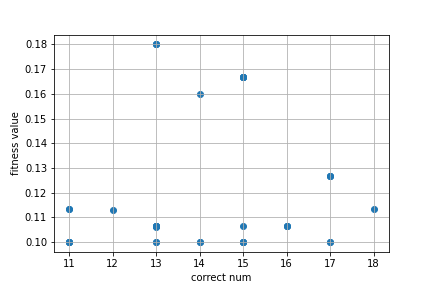
\includegraphics[scale=0.45]{img.png}
		\caption{SVMにおける散布図\label{fig:ex2_1}}
	\end{center}
\end{figure}


\begin{figure}[h]
	\begin{center}
		\centering
		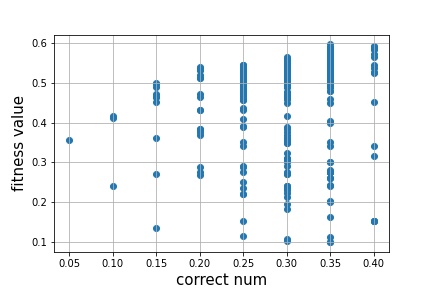
\includegraphics[scale=0.45]{img2.png}
		\caption{RandomForestにおける散布図\label{fig:ex2_2}}
	\end{center}
\end{figure}


\begin{figure}[h]
	\begin{center}
		\vspace*{-7mm}
		\hspace*{-8mm}
		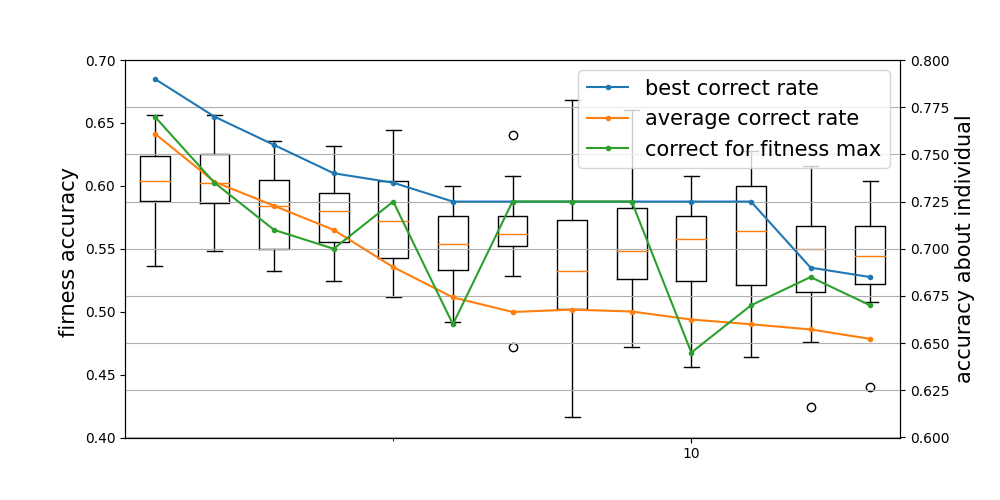
\includegraphics[height=65mm,width=110mm]{graph.png}
		\caption{SVM結果\label{fig:ex1}}
	\end{center}
\end{figure}

\begin{figure}[h]
	\begin{center}
		\vspace*{-7mm}
		\hspace*{-8mm}
		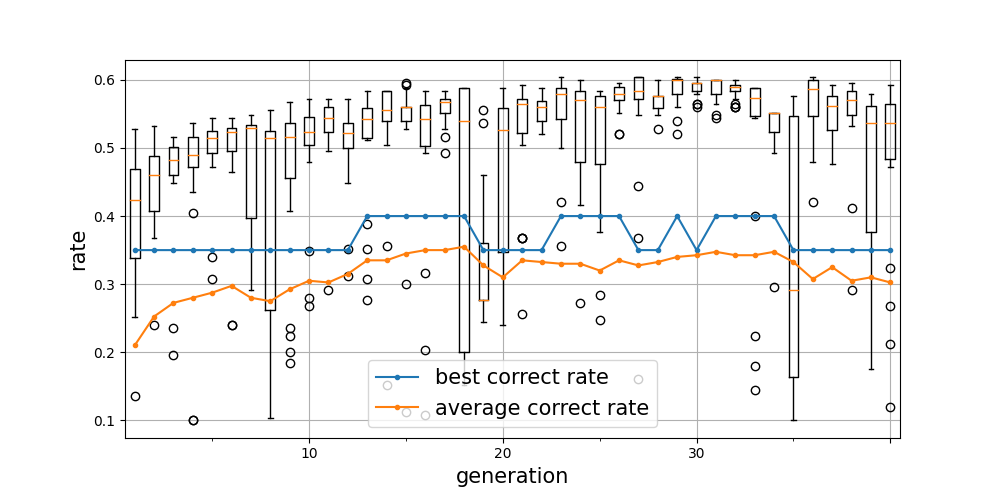
\includegraphics[height=65mm,width=110mm]{graph2.png}
		\caption{RandomForest結果\label{fig:ex2}}
	\end{center}
\end{figure}

\section{来週の課題}
	\begin{itemize}
		\item FixMatchの時間短縮(modelの縮小,最終層のみの学習など)
	\end{itemize}


\end{document}


